%
%Не забыть:
%--------------------------------------
%Вставить колонтитулы, поменять название на титульнике



%--------------------------------------

\documentclass[a4paper, 12pt]{article} 

%--------------------------------------
%Russian-specific packages
%--------------------------------------
%\usepackage[warn]{mathtext}
\usepackage[T2A]{fontenc}
\usepackage[utf8]{inputenc}
\usepackage[english,russian]{babel}
\usepackage[intlimits]{amsmath}
\usepackage{esint}
%--------------------------------------
%Hyphenation rules
%--------------------------------------
\usepackage{hyphenat}
\hyphenation{ма-те-ма-ти-ка вос-ста-нав-ли-вать}
%--------------------------------------
%Packages
%--------------------------------------
\usepackage{amsmath}
\usepackage{amssymb}
\usepackage{amsfonts}
\usepackage{amsthm}
\usepackage{latexsym}
\usepackage{mathtools}
\usepackage{etoolbox}%Булевые операторы
\usepackage{extsizes}%Выставление произвольного шрифта в \documentclass
\usepackage{geometry}%Разметка листа
\usepackage{indentfirst}
\usepackage{wrapfig}%Создание обтекаемых текстом объектов
\usepackage{fancyhdr}%Создание колонтитулов
\usepackage{setspace}%Настройка интерлиньяжа
\usepackage{lastpage}%Вывод номера последней страницы в документе, \lastpage
\usepackage{soul}%Изменение параметров начертания
\usepackage{hyperref}%Две строчки с настройкой гиперссылок внутри получаеммого
\usepackage[usenames,dvipsnames,svgnames,table,rgb]{xcolor}% pdf-документа
\usepackage{multicol}%Позволяет писать текст в несколько колонок
\usepackage{cite}%Работа с библиографией
\usepackage{subfigure}% Человеческая вставка нескольких картинок
\usepackage{tikz}%Рисование рисунков
\usepackage{float}% Возможность ставить H в положениях картинки
% Для картинок Моти
\usepackage{misccorr}
\usepackage{lscape}
\usepackage{cmap}



\usepackage{graphicx,xcolor}
\graphicspath{{Pictures/}}
\DeclareGraphicsExtensions{.pdf,.png,.jpg}

%----------------------------------------
%Список окружений
%----------------------------------------
\newenvironment {theor}[2]
{\smallskip \par \textbf{#1.} \textit{#2}  \par $\blacktriangleleft$}
{\flushright{$\blacktriangleright$} \medskip \par} %лемма/теорема с доказательством
\newenvironment {proofn}
{\par $\blacktriangleleft$}
{$\blacktriangleright$ \par} %доказательство
%----------------------------------------
%Список команд
%----------------------------------------
\newcommand{\grad}
{\mathop{\mathrm{grad}}\nolimits\,} %градиент

\newcommand{\diver}
{\mathop{\mathrm{div}}\nolimits\,} %дивергенция

\newcommand{\rot}
{\ensuremath{\mathrm{rot}}\,}

\newcommand{\Def}[1]
{\underline{\textbf{#1}}} %определение

\newcommand{\RN}[1]
{\MakeUppercase{\romannumeral #1}} %римские цифры

\newcommand {\theornp}[2]
{\textbf{#1.} \textit{ #2} \par} %Написание леммы/теоремы без доказательства

\newcommand{\qrq}
{\ensuremath{\quad \Rightarrow \quad}} %Человеческий знак следствия

\newcommand{\qlrq}
{\ensuremath{\quad \Leftrightarrow \quad}} %Человеческий знак равносильности

\renewcommand{\phi}{\varphi} %Нормальный знак фи

\newcommand{\me}
{\ensuremath{\mathbb{E}}}

\newcommand{\md}
{\ensuremath{\mathbb{D}}}



%\renewcommand{\vec}{\overline}




%----------------------------------------
%Разметка листа
%----------------------------------------
\geometry{top = 3cm}
\geometry{bottom = 2cm}
\geometry{left = 1.5cm}
\geometry{right = 1.5cm}
%----------------------------------------
%Колонтитулы
%----------------------------------------
\pagestyle{fancy}%Создание колонтитулов
\fancyhead{}
%\fancyfoot{}
\fancyhead[R]{\textsc{Подготовка к экзамену}}%Вставить колонтитул сюда
%----------------------------------------
%Интерлиньяж (расстояния между строчками)
%----------------------------------------
%\onehalfspacing -- интерлиньяж 1.5
%\doublespacing -- интерлиньяж 2
%----------------------------------------
%Настройка гиперссылок
%----------------------------------------
\hypersetup{				% Гиперссылки
	unicode=true,           % русские буквы в раздела PDF
	pdftitle={Заголовок},   % Заголовок
	pdfauthor={Автор},      % Автор
	pdfsubject={Тема},      % Тема
	pdfcreator={Создатель}, % Создатель
	pdfproducer={Производитель}, % Производитель
	pdfkeywords={keyword1} {key2} {key3}, % Ключевые слова
	colorlinks=true,       	% false: ссылки в рамках; true: цветные ссылки
	linkcolor=blue,          % внутренние ссылки
	citecolor=blue,        % на библиографию
	filecolor=magenta,      % на файлы
	urlcolor=cyan           % на URL
}
%----------------------------------------
%Работа с библиографией (как бич)
%----------------------------------------
\renewcommand{\refname}{Список литературы}%Изменение названия списка литературы для article
%\renewcommand{\bibname}{Список литературы}%Изменение названия списка литературы для book и report
%----------------------------------------
\begin{document}
	\begin{titlepage}
		\begin{center}
			$$$$
			$$$$
			$$$$
			$$$$
			{\Large{НАЦИОНАЛЬНЫЙ ИССЛЕДОВАТЕЛЬСКИЙ УНИВЕРСИТЕТ}}\\
			\vspace{0.1cm}
			{\Large{ВЫСШАЯ ШКОЛА ЭКОНОМИКИ}}\\
			\vspace{0.25cm}
			{\large{Факультет физики}}\\
			\vspace{5.5cm}
			{\Huge\textbf{{Подготовка к экзамену}}}\\%Общее название
			\vspace{1cm}
			\vspace{2cm}
			{Работу выполнил студент 3 курса}\\
			{Захаров Сергей Дмитриевич}
			\vfill
			
\includegraphics[width = 0.2\textwidth]{HSElogo}\\
			\vfill
			Москва\\
			2020
		\end{center}
	\end{titlepage}
	
\tableofcontents

\newpage

\section{Симметрия кристаллов, что это такое? Основные операции симметрии. Взаимодействие операций симметрии}

\textbf{Симметрия кристаллов} --- их свойство совмещаться самим с собой при различных преобразованиях, например поворотах вокруг осей, отражениях в плоскостях или точках (инверсия), параллельном переносе, или же комбинации этих операций.

В результате симметрических преобразований различные части или объект полностью самосовмещаются.

Если смотреть больше, то симметрия --- инвариантность объектов при линейных преобразованиях системы координат, которую мы используем для описания объекта, т.е. операция $\hat{\mathbf{G}}(x, y, z) \rightarrow [X, Y, Z]$ операция симметрии если:

\begin{equation}
	\hat{\mathbf{G}} [f(x, y, z)] = f(X, Y, Z)
\end{equation}

Симметрия кристаллов выделяется с помощью элементов симметрии:

\begin{enumerate}
	\item Центра симметрии
	
	\item Плоскостей симметрии
	
	\item Осей симметрии
\end{enumerate}

А также особой симметрии: трансляционной.

\subsubsection*{Центр симметрии}

Центр симметрии (инверсии) связывает противоположные инверсионно равные (или обращено равные) части кристалла. Он совпадает с геометрическим центром кристалла. От слова Centrum он обозначается буквой С (по символике Бравэ) или $\bar{1}$ (по интернациональной символике).

При наличии центра симметрии все диаметрально противоположные грани и ребра кристалла должны быть попарно инверсионно равны и параллельны. Это на пальцах можно проверить, положив кристалл на горизонтальную плоскость стола. Если все грани и ребра кристалла попарно параллельны и инверсионно равны, центр симметрии в кристалле есть. Если центр симметрии отсутствует, то в таком кристалле сверху окажется вершина, ребро, наклонная или параллельная, но не равная нижней, грань.

\subsubsection*{Плоскость симметрии}

Плоскость симметрии делит кристалл на две зеркально-равные половины. Плоскость симметрии связывает зеркально равные части кристалла. От слова Planum обозначается буквой Р (по Бравэ), от слова mirror (зеркало, отражать) обозначается буквой m (интернационально), графически обозначается сдвоенной линией (как двухсторонне зеркало).

Для определения плоскости симметрии кристалл мысленно рассекается плоскостью, проходящей через его центр. Если при этом слева и справа от плоскости симметрии все части кристалла (грани, ребра, вершины) будут повторяться как предмет и его зеркальное отображение, то такая плоскость будет являться плоскостью симметрии.
В прямоугольнике (см. рисунок \ref{fig:rect}) можно провести только две плоскости симметрии. Плоскость, делящая прямоугольник на две равные части, но не зеркально, не является плоскостью симметрии.

\begin{figure}[H]
	\centering
	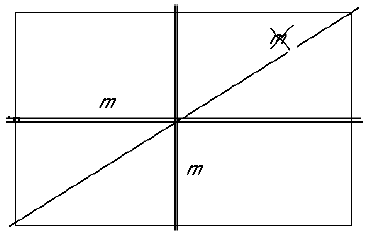
\includegraphics[width=0.5\linewidth]{Rectangle}
	\caption{Плоскости симметрии прямоугольника}
	\label{fig:rect}
\end{figure}

Куб (см. рисунок \ref{fig:cube}) имеет 9 плоскостей симметрии: три- координатных Р (слева), шесть диагональных Р (справа).

\begin{figure}[H]
	\centering
	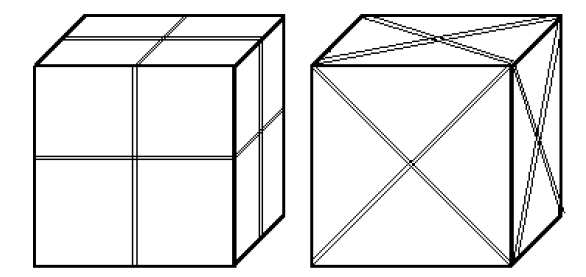
\includegraphics[width=0.5\linewidth]{Cube}
	\caption{Плоскости симметрии куба}
	\label{fig:cube}
\end{figure}

\subsubsection*{Оси симметрии}

Ось симметрии - это линии, которые симметрично связывает конгруэнтно равные (совместимо равные) части кристалла.
Вокруг оси симметрии на равных угловых и линейных расстояниях располагаются конгруэнтно равные части кристалла, так что при полном повороте вокруг оси (на 360$^\circ$) они повторяются $n$ раз. Такие оси называют поворотными осями симметрии $n$-го порядка.

В некоторых кристаллах, помимо поворотных осей симметрии, могут быть инверсионные оси симметрии, в которых операция симметричного поворота вокруг оси совмещается с операцией симметричного отражения в центре кристалла. Порядок инверсионной оси удваивается по сравнению с порядком поворотной оси.

По Браве от слова Linie они обозначаются L$n$ (читается - ось симметрии $n$-го порядка). В кристаллах могут быть поворотные оси симметрии первого L1, второго L2, третьего L3, четвертого L4, шестого L6 порядков и инверсионные оси симметрии Li1, Li2, Li3, Li4, Li6. Кроме того, Li1 = С, Li2 = P, Li3 = L3C, Li4 = L2, Li6 = L3P (про запрем L5 см. далее в операции трансляции).

По интернациональной символике поворотные оси симметрии обозначаются числом, указывающим их порядок, т.е. 1, 2, 3, 4 и 6, а инверсионные оси симметрии --- $\bar{1}$, $\bar{2}$, $\bar{3}$, $\bar{4}$ и $\bar{6}$.

Графически оси симметрии обозначаются многоугольником, число углов которого равно порядку оси симметрии.

В кубе: ЗL4 - (3 оси симметрии 4-го порядка) проходят через середины противоположных квадратных граней; 4L3 - (4 оси симметрии 3-го прядка) проходят через противоположные вершины; 6L2 - (6 осей симметрии 2-го прядка) проходят через середины противоположных ребер куба.

Для объяснения ''на пальцах'' полезно запомнить, что концы осей симметрии в кристаллах могут выходить через вершины, через центры граней и через середины ребер. Следовательно, при определении осей симметрии именно за эти элементы и нужно брать кристалл двумя пальцами и вращать его вокруг этой оси.

\subsubsection*{Операция трансляции}

Если решетка кристалла состоит из повторяющихся в пространстве элементарных ячеек, то существует еще \textbf{трансляционная симметрия}, т.е. наличие некоторого \textit{вектора трансляции}, с помощью которого можно построить всю бесконечную кристаллическую решетку путем переноса одной элементарной ячейки.

Трансляционная симметрия вкупе с операциями поворота и отражения в плоскости и в точке приводит к возникновению таких элементов симметрии как винтовая ось, инверсионная ось, плоскость скользящего отражения.

Кроме того, наличие трансляционной симметрии запрещает существование оси пятого порядка. Пусть у нас есть двумерная решетка, которая состоит из узловых рядов $A_1, A_2$, период транслции вдоль этого ряда есть $t$. Положим также, что перпендикулярно исследуемой плоскости проходит $n$-кратная ось симметрии (см. рисунок \ref{fig:nol5}). Тогда $A_1$ переходит в точку $B_1$, $A_2$ --- в $B_2$, угол поворота из кратности оси симметрии:

\begin{equation}
	\alpha = \frac{2\pi}{n}
\end{equation}

\begin{figure}[H]
	\centering
	\includegraphics[width=0.7\linewidth]{nol5}
	\caption{К выводу запрета на L5}
	\label{fig:nol5}
\end{figure}

Понятно, что $B_1$ и $B_2$ определят ряд решетки, параллельный ряду $A_1$ --- $A_2$. Тогда расстояние между точками $B_1$ и $B_2$ неминуемо должно быть кратно периоду трансляции $t$. По построению из трапеции:

\begin{equation}
	B_1B_2 = t - 2t\cos\alpha = \xi t \qrq \cos\alpha = \frac{1 - \xi}{2}
	\label{eq:nocos}
\end{equation}

Ясно, что на косинус существует условие его принадлежности к интервалу [$-1$; 1]. Проверив все возможные $\xi$, убедимся, что $\alpha = 2\pi/5$ (соответствует пятому порядку оси симметрии) соответствующего косинуса из \ref{eq:nocos} не находится. Кроме того, таким же образом оказывается, что порядка выше шестого быть также не может.

\section{Методы изображения кристаллов. Стереографические проекции. Как они устроены?}

%Для изображения элементов кристаллической решетки используется система координат, приведенная на рисунке \ref{fig:coord}. В общем случае она может быть непрямоугольной.
%
%\begin{figure}[H]
%	\centering
%	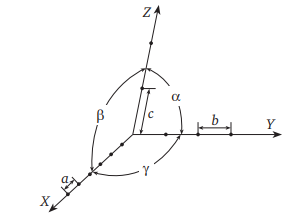
\includegraphics[width=0.5\linewidth]{Coordinate_axes}
%	\caption{Кристаллографическая система координат. $a$, $b$, $c$ --- масштабы по осям координат, $\alpha$, $\beta$, $\gamma$ --- углы между осями.}
%	\label{fig:coord}
%\end{figure}
%
%В такой СК положение узла задается вектором:
%
%\begin{equation}
%	\mathbf{r_j} = \mathbf{a} m + \mathbf{b} n + \mathbf{c} p
%\end{equation}
%
%Здесь $m$, $n$, $p$ --- целые.

Потенциально возможно изображать кристалл просто в изометрии, однако это неудобно по чисто человеческим причинам (требуется пространственное воображение и все такое), а также по причине отсутствия правильного представления об угловых параметрах кристалла. По этой причине используется метод кристаллографических проекций, для которого все плоскости заменяются нормалями к ним. После этого мы параллельно переносим их таким образом, чтобы они все пересекались в одной точке. Полученная совокупность нормалей называется \textbf{кристаллографическим комплексом}

После этого вокруг точки пересечения строится сфера. Сфера, по очевидным соображениям, ''протыкается'' нормалями, образуя так называемую \textbf{сферическую проекцию} плоскостей, которые мы заменили нормалями. Фактически мы получаем эдакий глобус, с помощью которого теперь уже можно измерять углы между плоскостями.

Этот обход однако не решает проблему использования изометрии, поэтому сферу необходимо спроецировать на плоскость. Сделать это можно по-разному, однако применение нашел способ проектирования на экваториальную плоскость (такие проекции называются \textbf{стереографическими}). Схема их построения приведена на рисунке \ref{fig:stero_ex}. 

\begin{figure}[H]
	\centering
	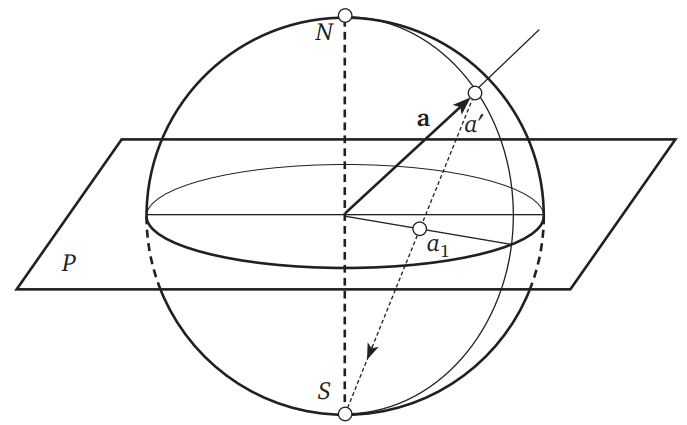
\includegraphics[width=0.7\linewidth]{Stereo_example}
	\caption{К построению стереографической проекции. Точка $a_1$ есть \textbf{стереографическая проекция кристаллографической плоскости}.}
	\label{fig:stero_ex}
\end{figure}

Указанный метод, с одной стороны, позволяет проводить непосредственные измерения угловых параметров решетки, а с другой --- позволяет сразу же видеть наличие или отсутствие той или иной симметрии.

Для того, чтобы удобно проводить угловые измерения, используется объект, называемый \textbf{сетка Вульфа} --- фактически, стереографическая проекция всех параллелей и меридианов на ''глобусе'' с шагом 2$^\circ$. Он может быть, например, исполнен на прозрачном материале и накладываться на стереографическую проекцию.

\section{Определить индексы Миллера плоскости, проходящей через две телесные диагонали куба}

К сожалению, верстать картинки пока что находится за гранью моего сознания, поэтому задача приложена как скан.



\end{document}